\frame[plain]{\titlepage}
\frame{\frametitle{Outline}\tableofcontents}

\section{Problem - Nonlinear Real Arithmetic}
\subsection{Search Space of SMT(NRA)}

\begin{frame}
    \frametitle{Syntax of SMT(NRA)}
    
    polynomial: $p ::= x \mid c \mid p + p \mid p - p \mid p \times p$

    atoms: $a ::= b \mid p = 0 \mid p > 0 \mid p < 0$

    formula: $f ::= a \mid \neg f \mid f \wedge f \mid f \vee f $

    \vspace{0.4cm}

    SMT: Determine whether the formula is satisfied by some assignment (local search focuses), or prove unsat

    \vspace{0.4cm}

    Example:
    \\
    $x^2 + y^2 \le 1 \wedge x + y < 1 \wedge x + z > 0$
    \\
    assignment with $\left\{x \rightarrow 0, y \rightarrow 0, z \rightarrow 1\right\}$ satisfies all clauses.
\end{frame}

\begin{frame}{Fragment of Local Search}

    \begin{onlyenv}<1>
    \begin{algorithm}[H]
    \SetKwBlock{Begin}{}{}
    \SetAlgoLined
    \SetKwInOut{Input}{Input}
\SetKwInOut{Output}{Output}
\Input{A set of clauses $F$}
\Output{An assignment of variables that satisfy $F$, or failure}
Initialize assignment to variables\;
\While{$\top$}{
    \If{all clauses satisfied}{
        \Return{success with assignment\;}
    }
    \If{time or step limit reached}{
        \Return{failure\;}
    }
    Critical move procedure.
}
\caption{Basic Fragment of Local Search}
    \end{algorithm}
    \end{onlyenv}
    
    \begin{onlyenv}<2>
    \begin{algorithm}[H]
    \SetKwBlock{Begin}{}{}
        $\mathit{var,new\_value,score} \leftarrow$ best move according to make-break score\;
    \If{score $>$ 0}{
        Perform move, assigning $\mathit{var}$ to $\mathit{new\_value}$\;
    }
    \Else{
        Update clause weight according to PAWS scheme\;
        \Repeat{3 times}{
            $\mathit{cls} \leftarrow$ random unsatisfied clause\;
            $\mathit{var,new\_value,score} \leftarrow$ critical move making $\mathit{cls}$ satisfied\;
            \If{score $\neq$ $-\infty$}{
                Perform move, assigning $\mathit{var}$ to $\mathit{new\_value}$\;
            }
        }
        \If{no move performed in previous loop}{
            Change assignment of some variable in some unsatisfied clause\;
        }
    }
    \end{algorithm}
    \end{onlyenv}
    \end{frame}
    

\begin{frame}
    \frametitle{Local Search for SAT and SMT}

    \begin{center}
        \begin{tabular}{|c|c|c|}
            \hline
            \diagbox{LS}{Problem}&SAT&SMT\\
            \hline
            Operation (Move)&Flip&Critical Move\\
            \hline
            Score Definition & \multicolumn{2}{c|}{Weighted unsat clauses}\\
            \hline
            Score Computation & Cached score& No Caching, time costly\\
            \hline 
            \end{tabular}
    \end{center}

    \textbf{What LS for SAT brings us: }\\
    Maintain scoring information after each iteration.\\
    \textbf{Difficulty:}\\
    Predetermine critical move shift value.\\
    \textbf{Our Solution:}\\
    Introduce Scoring Boundaries.
\end{frame}

\subsection{Current Existing Methods}

\section{Incremental Computation of Variable Scores}
\subsection{Scoring Boundary for Arithmetic Variable}

\begin{frame}{Critical Move Value ? Interval!}
    Reference introduces multiple values choices for critical move, resulting in different scores.\\
    Actually, \textbf{interval} brings the difference.
\end{frame}

\begin{frame} 
    \frametitle{Boundary}

    \textbf{Brief. }Given an arithmetic variable, maintain critical move scores for specific moving intervals.
    \\
    \textbf{Definition. } 123
    \\
    \textbf{Example. }\\
    Assume boundary for variable $v$ is

    % \begin{block}{Pythagorean theorem}
    %     \vspace*{-\baselineskip}\setlength\belowdisplayshortskip{0.6pt}
    %     $$a^2 + b^2 = c^2$$
    %     % \vspace*{-\baselineskip}\setlength\belowdisplayshortskip{0.1pt}
    %     where c represents the length of the hypotenuse and 
    %     a and b the lengths of the triangle's other two sides.
    % \end{block}
    
    \begin{alertblock}{Remark}
        \begin{itemize}
            \item the environment above is \alert{block}
            \item the environment here is \alert{alertblock}
        \end{itemize}
    \end{alertblock}
\end{frame}

\begin{frame}
    \frametitle{Boundary Example}
    Assume boundary for variable $v$ as below:\\
    \vspace{1cm}
    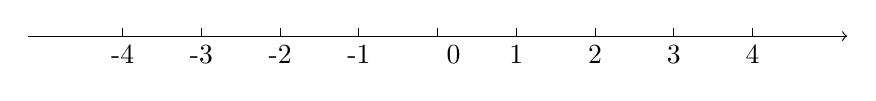
\begin{tikzpicture}
        %画x和y轴坐标
        \draw[->] (-5.2,0)--(5.2,0);
        %画刻度
        \foreach \x in {0,1,...,8}
        {
            \draw[xshift=\x cm] (-4,0) -- (-4,0.1);
        };  
        %标坐标原点
        \node[below] at (0.2,0){0};
        %标x轴刻度值
        \foreach \x in {-4,-3,...,-1}
            \node[below] at(\x,0){\x};
        \foreach \y in {1,2,...,4}
            \node[below] at(\y,0){\y};
        \end{tikzpicture}
\end{frame}

\subsection{Incremental Computation}

\begin{frame}{Computation of Boundary (Incremental)}
    \scriptsize
    \begin{algorithm}[H]
        \KwData{this text}
        \KwResult{how to write algorithm with \LaTeX2e }
        initialization\;
        \While{not at end of this document}{
            read current\;
            \eIf{understand}{
            go to next section\;
            current section becomes this one\;
            }{
            go back to the beginning of current section\;
            }
        }
        \caption{How to write algorithms
        (copied from \href{https://en.wikibooks.org/wiki/LaTeX/Algorithms}{here})}
        \end{algorithm}
\end{frame}

\section{Temporary Relaxation of Equality Constraints}

\subsection{Difficulty in Local Search}

\begin{frame}{Equality Constraints in Local Search}
    \begin{minipage}{0.5\linewidth}
        \begin{figure}[h]
            \includegraphics[width=\textwidth]{imgs/pythagorean.jpg}
        \end{figure}
    \end{minipage}%
    \hfill
    \begin{minipage}{0.4\linewidth}
        \begin{enumerate}
            \item item
            \item another
            \item more
            \begin{itemize}
                \item first
                \item second
                \item third
            \end{itemize}
        \end{enumerate}
    \end{minipage}
\end{frame}

\subsection{Relaxation Method}

\begin{frame}{Relaxation}
    \begin{columns}
        \column{0.5\textwidth}
        This is a text in first column.
        $$E=mc^2$$
        \begin{itemize}
        \item First item
        \item Second item
        \end{itemize}
        
        \column{0.5\textwidth}
        \begin{block}{first block}
            columns achieves splitting the screen
        \end{block}
        \begin{block}{second block}
            stack block in columns
        \end{block}
        
    \end{columns}
\end{frame}

\begin{frame}{Relaxation (CAD view)}
    
\end{frame}

\begin{frame}{Restore}
    
\end{frame}

\section{Implementation Detail}
\subsection{Look-ahead}
\subsection{Other}

\section{Conclusion}

\begin{frame}{End}
    The last page.
\end{frame}